% -----------------------------------------------
% Template for SMC 2019
% adaed from the template for SMC 2018
% -----------------------------------------------

\documentclass{article}
\usepackage{smc2019}
\usepackage{times}
\usepackage{ifpdf}
\usepackage[english]{babel}
\usepackage{cite}
\usepackage[utf8]{inputenc}

%\usepackage{graphicx}
%\usepackage{amssymb,amsmath} 
\usepackage{balance}

\usepackage{color}
%\usepackage{hyperref}
\usepackage[nocenter]{qtree}
\usepackage{tree-dvips}
\usepackage{listings}

\definecolor{lightgrey}{rgb}{0.95,0.95,0.95}

\newcommand{\IS}		{INScore}
\newcommand{\exemple}	{\vspace*{1mm}\hspace*{-4mm}\textbf{Example :}}

\definecolor{mygrey}{gray}{0.93}
\newcommand{\code}	[2][0.9]		{\vspace{0mm}\begin{center}\colorbox{mygrey}{
							\begin{minipage}[t]{#1\columnwidth} 
							{\small \texttt{#2}}
							\end{minipage}}\end{center}}
\newcommand{\op}	[1]		{\vspace{0mm}\begin{center}\colorbox{mygrey}{
							\begin{minipage}[t]{0.9\columnwidth} 
							{\small \texttt{#1}}
							\end{minipage}}\end{center}}
\newcommand{\nulltree}	{\ensuremath{\varnothing}}
\newcommand{\seq}		{\ensuremath{|}}
\newcommand{\paral}		{\ensuremath{\parallel}}
\newcommand{\foret}		{\ensuremath{\phi}}
\newcommand{\toforet}	{\ensuremath{\mathcal{F}}}
\newcommand{\expand}	{\ensuremath{\rightsquigarrow}}
\newcommand{\transform}	{\ensuremath{\xi}}
\newcommand{\binop}		{$op$}
\newcommand{\logop}		{$lop$}
\newcommand{\ftree}		{ftree}
\newcommand{\etc}		{…}

\newcommand{\nexpand}	{\ensuremath{\varepsilon}}
\newcommand{\ula}		{\hspace*{8mm}}
\newcommand{\ulb}		{\hspace*{4mm}}
\newcommand{\ulc}		{\hspace*{37mm}}
\newcommand{\uld}		{\hspace*{9mm}}


%%%%%%%%%%%%%%%%%%%%%%%% Some useful packages %%%%%%%%%%%%%%%%%%%%%%%%%%%%%%%
%%%%%%%%%%%%%%%%%%%%%%%% See related documentation %%%%%%%%%%%%%%%%%%%%%%%%%%
\usepackage{amsmath} % popular packages from Am. Math. Soc. Please use the 
\usepackage{amssymb} % related math environments (split, subequation, cases,
\usepackage{amsfonts}% multline, etc.)
%\usepackage{bm}      % Bold Math package, defines the command \bf{}
%\usepackage{paralist}% extended list environments
%%subfig.sty is the modern replacement for subfigure.sty. However, subfig.sty 
%%requires and automatically loads caption.sty which overrides class handling 
%%of captions. To prevent this problem, preload caption.sty with caption=false 
%\usepackage[caption=false]{caption}
%\usepackage[font=footnotesize]{subfig}

% ====================================================
% ================ Define title and author names here ===============
% ====================================================
%user defined variables
\def\papertitle{A Tree Based Language for Music Score Description.}
\def\firstauthor{D. Fober}
\def\secondauthor{Y. Orlarey}
\def\thirdauthor{S. Letz}
\def\fourthauthor{R. Michon}

% adds the automatic
% Saves a lot of output space in PDF... after conversion with the distiller
% Delete if you cannot get PS fonts working on your system.

% pdf-tex settings: detect automatically if run by latex or pdflatex
\newif\ifpdf
\ifx\pdfoutput\relax
\else
   \ifcase\pdfoutput
      \pdffalse
   \else
      \pdftrue
  \fi
\fi

\ifpdf % compiling with pdflatex
  \usepackage[pdftex,
    pdftitle={\papertitle},
    pdfauthor={\firstauthor, \secondauthor, \thirdauthor},
    bookmarksnumbered, % use section numbers with bookmarks
    pdfstartview=XYZ % start with zoom=100% instead of full screen; 
                     % especially useful if working with a big screen :-)
   ]{hyperref}
  %\pdfcompresslevel=9

  \usepackage[pdftex]{graphicx}
  % declare the path(s) where your graphic files are and their extensions so 
  %you won't have to specify these with every instance of \includegraphics
  \graphicspath{{./figures/}}
  \DeclareGraphicsExtensions{.pdf,.jpeg,.png}

  \usepackage[figure,table]{hypcap}

\else % compiling with latex
  \usepackage[dvips,
    bookmarksnumbered, % use section numbers with bookmarks
    pdfstartview=XYZ % start with zoom=100% instead of full screen
  ]{hyperref}  % hyperrefs are active in the pdf file after conversion

  \usepackage[dvips]{epsfig,graphicx}
  % declare the path(s) where your graphic files are and their extensions so 
  %you won't have to specify these with every instance of \includegraphics
  \graphicspath{{./figures/}}
  \DeclareGraphicsExtensions{.eps}

  \usepackage[figure,table]{hypcap}
\fi

%setup the hyperref package - make the links black without a surrounding frame
\hypersetup{
    colorlinks,%
    citecolor=black,%
    filecolor=black,%
    linkcolor=black,%
    urlcolor=black
}


% ====================================================
% ================ Title and author info starts here ===============
% ====================================================
% Title.
% ------
\title{\papertitle}

% Authors
% Please note that submissions are anonymous, therefore 
% authors' names should not be VISIBLE in your paper submission.
% They should only be included in the camera-ready version of accepted papers.
% uncomment and use the appropriate section (1, 2 or 3 authors)
%
% Single address
% To use with only one author or several with the same address
% ---------------
\oneauthor
   {D. Fober \quad Y. Orlarey \quad S. Letz \quad R. Michon} {Grame-CNCM \\
  Lyon - France \\ %
     {\tt {\small \{fober, orlarey, letz, michon\}@grame.fr}}}

%Two addresses
% the default spacing is 1.5in, but this can be reduced to 0.5in or less, if needed
%--------------
% \twoauthors
%   {1.5in}
%   {\firstauthor} {Affiliation1 \\  %
%     {\tt \href{mailto:author1@unt.edu}{author1@unt.edu}}}
%   {\secondauthor} {Affiliation2 \\  %
%     {\tt \href{mailto:author2@unt.edu}{author2@unt.edu}}}

% Three addresses
% the default spacing is 0.5in, but this can be reduced to 0.3in or less, if needed
% --------------
% \threeauthors
%   {0.5in}
%   {\firstauthor} {Affiliation1 \\ %
%     {\tt \href{mailto:author1@smcnetwork.org}{author1@smcnetwork.org}}}
%   {\secondauthor} {Affiliation2 \\ %
%     {\tt \href{mailto:author2@smcnetwork.org}{author2@smcnetwork.org}}}
%   {\thirdauthor} { Affiliation3 \\ %
%     {\tt \href{mailto:author3@smcnetwork.org}{author3@smcnetwork.org}}}

% Four addresses
% the default spacing is 1.5in, but this can be reduced to 0.5in or less, if needed
% --------------
% \fourauthors
%   {1.5in}
%   {\firstauthor} {Grame \\ %
%     {\tt \href{mailto:fober@grame.fr}{fober@grame.fr}}}
%   {\secondauthor} {Grame \\ %
%     {\tt \href{mailto:orlarey@grame.fr}{orlarey@grame.fr}}}
%   {\thirdauthor} { Grame \\ %
%     {\tt \href{mailto:letz@grame.fr}{letz@grame.fr}}}
%   {\fourthauthor} { Grame \\ %
%     {\tt \href{mailto:michon@grame.fr}{michon@grame.fr}}}
%


% ====================================================
% =============== The document content starts here ===============
% ====================================================
\begin{document}
%
\capstartfalse
\maketitle
\capstarttrue
%
\begin{abstract}
The work presented is part of the \IS\ project, an environment for the design of augmented interactive music scores, oriented towards unconventional uses of music notation and representation, without excluding classical approaches. This environment is fully controllable using Open Sound Control [OSC] messages. \IS\ scripting language is an extended textual version of OSC messages that allows you to design scores in a modular and incremental way. This article presents a major revision of this scripting language, based on the description and manipulation of trees.
\end{abstract}
%

%-------------------------------------------------
\section{Introduction}\label{sec:introduction}

\IS \cite{Fober:12a} is a music notation and representation system initially designed to be driven by OSC messages \cite{OSC}. A textual version of these messages constitutes the storage format, which has been extended to a scripting language, \cite{Fober:13b} allowing greater flexibility in music scores design.

These extensions (introduction of variables, extended addresses, Javascript section, etc.) have nevertheless suffered from a rigidity inherent to an ad hoc and incremental design. As a result, a major revision of this language became necessary. It is based on the structure of the \IS\ model, which is a tree. 
The Figure \ref{tree1} gives an example of such hierarchy, which can be described in the current scripting language (i.e. OSC) by listing all branches from the root (figure~\ref{script1})
\begin{figure}[htbp]
\code{/ITL/scene/obj1 x 0;\\
/ITL/scene/obj1 y    0;\\
/ITL/scene/obj1 date 0;\\
/ITL/scene/obj2 x    0.5;\\
/ITL/scene/obj2 y    0.5;\\
/ITL/scene/obj2 date 1;
}
\caption{Messages to build the score in Figure \ref{tree1}.}
\label{script1}
\end{figure}


\begin{figure}[htbp]
\begin{center}
\Tree [ .ITL [ .scene 
	[ .obj1 [ .x 0 ] [ .y 0 ] [ .date 0 ] ] 
	[ .obj2 [ .x 0.5 ] [ .y 0.5 ] [ .date 1 ] ] ] 
]
\caption{A score sample including 2 objects $obj1$ and $obj2$, having a $x$, $y$, and $date$ attributes. The leaves of the tree are the values of the attributes.}
\label{tree1}
\end{center}
\end{figure}

There is a large number of musical score description languages (lilypond \cite{lilypond03}, guido \cite{hoos98}, MuseData \cite{Hewlett97}, MEI \cite{Roland_2002}, MusicXML \cite{good01}, abc, \footnote{\url{http://abcnotation.com/}} etc.) that are all turned towards common western music notation, and do not have programming capacity. 

However, the extension of some of these languages has been considered, in order to add \textit{programmability}. It includes, for example, operations to compose musical scores in guido \cite{fober12b}, or the scheme language as an extension of lilypond.

In addition, there are programming languages dedicated to music notation, like CMN \cite{Schottstaedt97} or ENP 
\cite{KUUSK06} which are in fact Lisp dialects, still oriented towards the common western notation.

OSC is defined as a communication protocol. However, programming capabilities have been added \cite{429}, in the form of \emph{functions} embedded in OSC messages, allowing structured functional communication between musical applications \cite{bresson:hal-01353794}. 

None of these approaches covers the very particular angle we have adopted: that of a language for describing music scores, based on the hierarchical structure of both the score and the OSC messages.

After some definitions, we will present the basic operations on trees and the corresponding grammar. We will then introduce mathematical operations on trees, the concepts of \emph{variables} and \emph{nodes in intention} and we'll present how this language is turned into OSC messages. The final section gives an example of the new language before concluding.


%-------------------------------------------------
\section{Definitions}

A tree is a data structure made up of nodes and edges without having any cycle. The tree with no nodes is called the null or empty tree. A tree that is not empty consists of a root node and potentially many levels of additional nodes that form a hierarchy \footnote{\href{https://en.wikipedia.org/wiki/Tree_(data_structure)}{from Wikipedia}}.


%---------------------------
\subsection{Terminology}

\begin{description}
 \setlength\itemsep{0.0em}
\item[Root]	The top node in a tree.
\item[Child]	A node directly connected to another node when moving away from the root.
\item[Parent]	The converse notion of a child.
\item[Leaf]	A node with no children.
\item[Edge]	The connection between one node and another.
\item[Path]	A sequence of nodes and edges connecting a node with a descendant.
\item[Forest]	A set of $n >= 0$ disjoint trees.
\end{description}

%---------------------------
\subsection{Trees}
A tree consists of a value (of some data type, possibly empty) and a forest (the subtrees of its children).
\code{f := [ t[1],..., t[k] ] \\
t :=  v f
}


%-------------------------------------------------
\section{Operations on Trees}

%-----------------------------
\subsection{Putting Trees in Sequence}
We will note \seq\ the sequencing operation of 2 trees. \\
Let 2 trees \texttt{t} and \texttt{t'} be defined as follows:
\op{f := [ t[1],\etc, t[k] ] \\
t :=  v f \\
\\
f' := [ t'[1],\etc, t'[k] ] \\
t' :=  v' f'
}
then
\op{t \seq\ t'  $\Rightarrow$  t" := v f" \\
f" := [ t[1] \seq\ t',\etc, t[k] \seq\ t']
}
with: 
\op{t :=  v [ \nulltree\ ]\\
t \seq\ t'  $\Rightarrow$  t" := v [ t' ]
}


%-----------------------------
\subsection{Putting Trees in Parallel}
We will note \paral\ the parallelisation operation. 
Let 2 trees \texttt{t} and \texttt{t'}:
\op{t \paral\ t'  $\Rightarrow$  t": \foret\ [ t, t' ]
}
\texttt{t"} is a tree which value \foret\ denotes a forest. 

We'll name \emph{\ftree} the type of tree whose value is \foret\ and we extend the sequencing operation to \emph{\ftree}\ as follows:
\op{t' :=  \foret\ f\\
t \ :=  v [ \nulltree\ ]\\
t \seq\ t'  $\Rightarrow$  t" := v f
}

Parallelisation applied to an \emph{\ftree} is distributed to children: 
\op{t :=  \foret\ [ t[1],\etc, t[k] ]\\
t' :=  v f\\
\\
t \paral\ t'  $\Rightarrow$  t" := \foret\ [t[1],\etc,t[k], t']\\
t' \paral\ t  $\Rightarrow$  t" := \foret\ [t', t[1],\etc,t[k]]
}



%-------------------------------------------------
\section{Grammar}\label{agram}

A tree is syntactically defined as follows:
\code{tree := value      \hspace*{8mm} $\to$ t := value [ \nulltree ] \\
\ula | tree tree         \hspace*{4mm} $\to$ t := tree \seq\ tree \\
\ula | / tree            \hspace*{9.7mm} $\to$ t := '/' \seq\ tree\\
\ula | tree , tree       \hspace*{0mm}  $\to$ t := tree \paral\ tree \\
\ula | ( tree )          \hspace*{6mm} $\to$ t := tree \\
\ula ;\\
}

\exemple

Figure~\ref{parsesample1} gives an example of this grammar with the tree built from this script. Figure~\ref{treesample1} shows this tree after evaluation of the sequencing ($seq$) and parallelisation ($par$) operations.

\begin{figure}[htbp]
\code{/a/b (c, (d e), f) (x 0), (y 1)}
\begin{center}
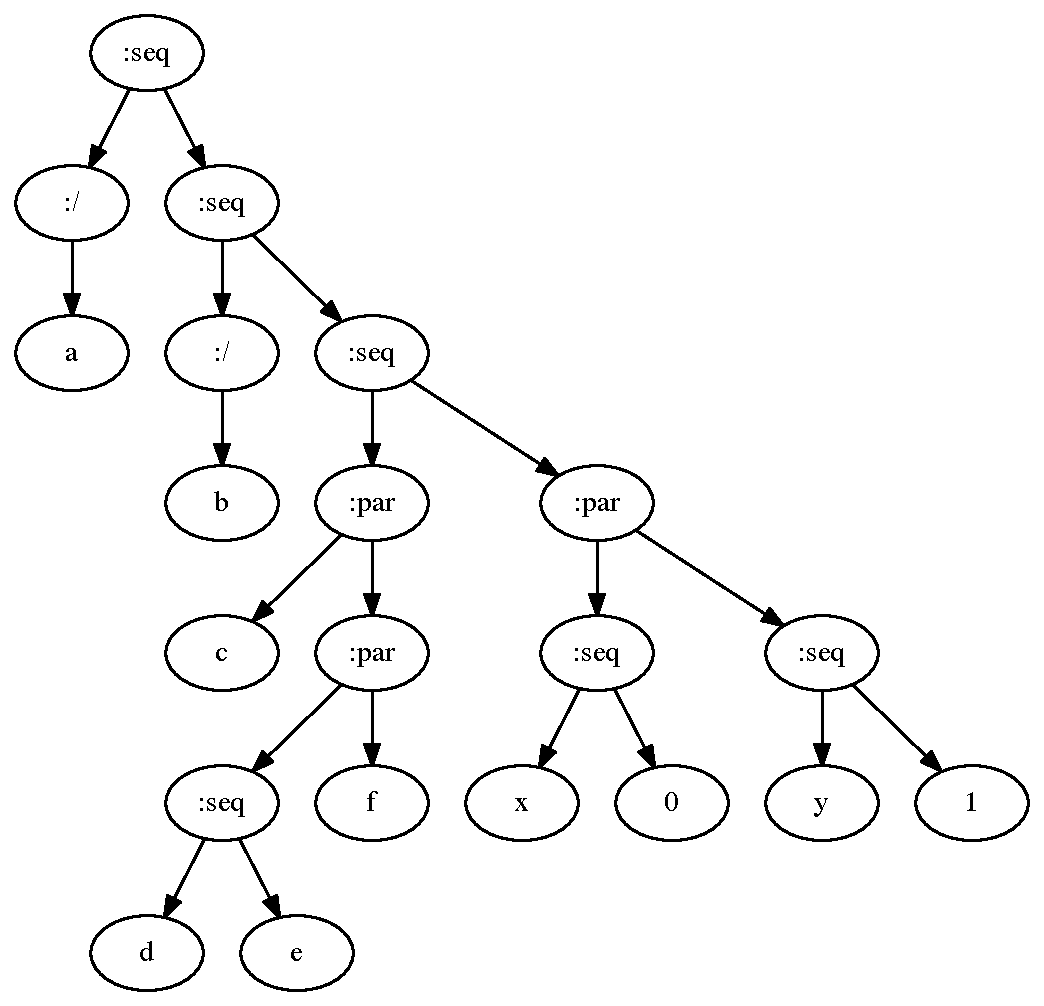
\includegraphics[width=0.7\columnwidth]{parse/sample1}
\caption{Tree built from the above script.}
\label{parsesample1}
\end{center}
\end{figure}

\begin{figure}[htbp]
\begin{center}
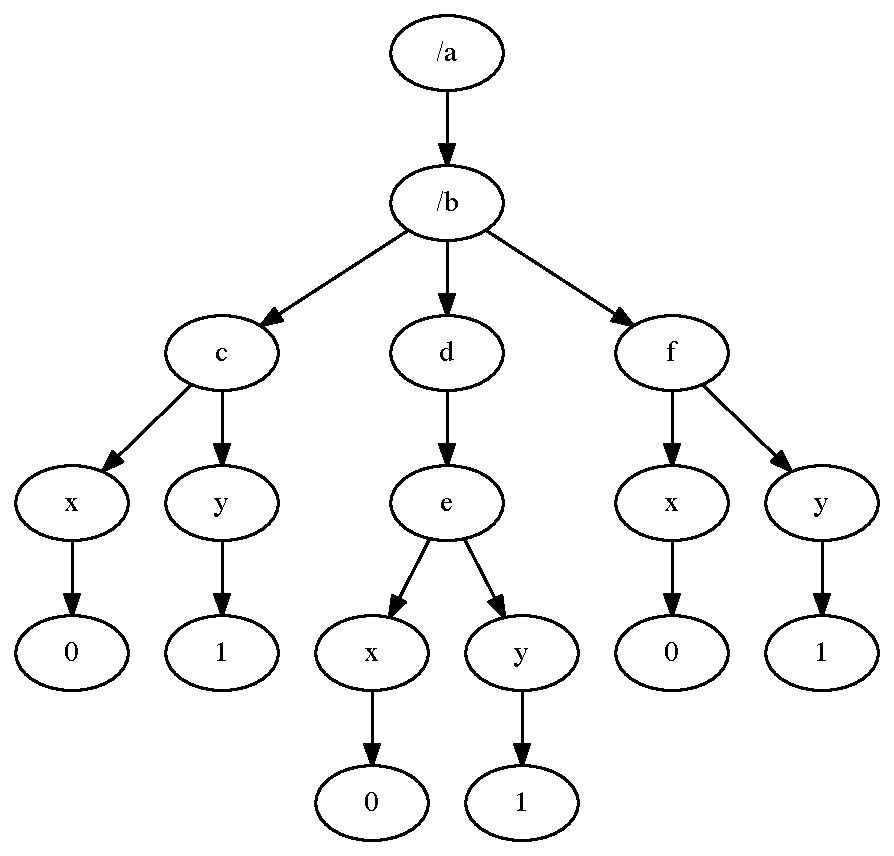
\includegraphics[width=0.6\columnwidth]{eval/sample1}
\caption{Tree generated by the evaluation of the $seq$ and $par$ operations in Figure \ref{parsesample1}.}
\label{treesample1}
\end{center}
\end{figure}

The nodes whose value is \emph{slash} (/) play a special role in the tree conversion to OSC messages. This role is described in section \ref{ssec:slash}.

%-------------------------------------------------
\section{Values and Evaluation}\label{sec:valeurs}

The nodes of a tree may contain literal values (i.e., text, number) or special values that are among the following types:
\begin{itemize}
 \setlength\itemsep{0.0em}
\item mathematical operators
\item variables
\item node in intention
\item slash (/)
\end{itemize}



%---------------------------
\subsection{Mathematical Operators}

Mathematical operations on trees are seen as operations on their values that preserve the subtrees. These operations are among:
\begin{itemize}
 \setlength\itemsep{0.0em}
\item arithmetic operations (+ - * / \%)
\item logical operations ($==$ $<$ $\leq$ $>$ $\geq$)
\item trigonometric function (sin, cos, tan, asin, acos, atan)
\item hyperbolic functions (sinh, cosh, tanh, asinh, acosh, atanh)
\item exponential and logarithmic functions (exp, log, log10, log2)
\item power and square root (pow, sqrt, cbrt)
\item miscellaneous  (min, max, rand)
\end{itemize}

We will designate these operations by \binop. Then:
\op{t :=  v f\\
t' := v' f'\\
\binop\ t t'  $\Rightarrow$  t":  (\binop\ v v') [ f $\cup$ f' ]  
}

\exemple

The script in Figure~\ref{parsesample2} generates the tree illustrated in Figure \ref{treesample2} after evaluation of the mathematical operations.

\begin{figure}[htbp]
\code{/a/b 	(c ((* (math.sin 1), 2)) 1) ,\\
\ulb		(d (math.pow 2.2, 0.4)),\\
\ulb		(e (>= 1, 1) (math.max 1, 2, 3, 4));}
\begin{center}
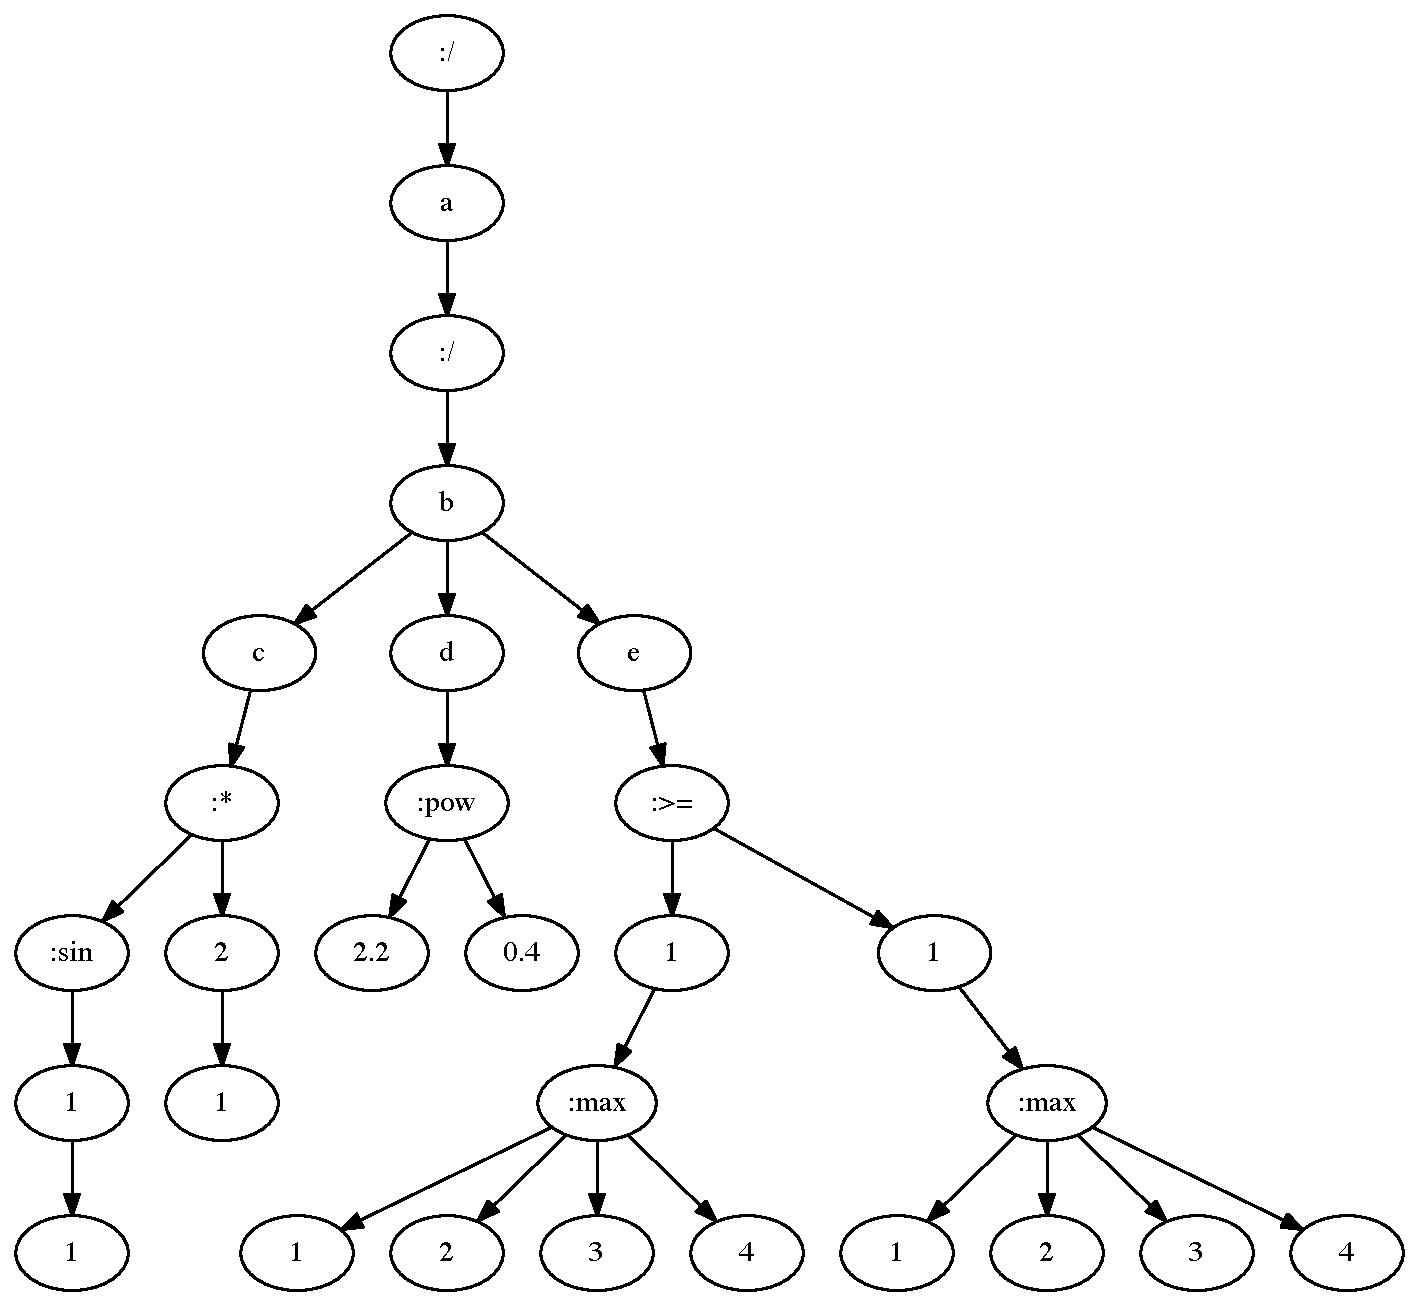
\includegraphics[width=0.72\columnwidth]{tree/sample3}
\caption{Tree built from the above script.}
\label{parsesample2}
\end{center}
\end{figure}

\begin{figure}[htbp]
\begin{center}
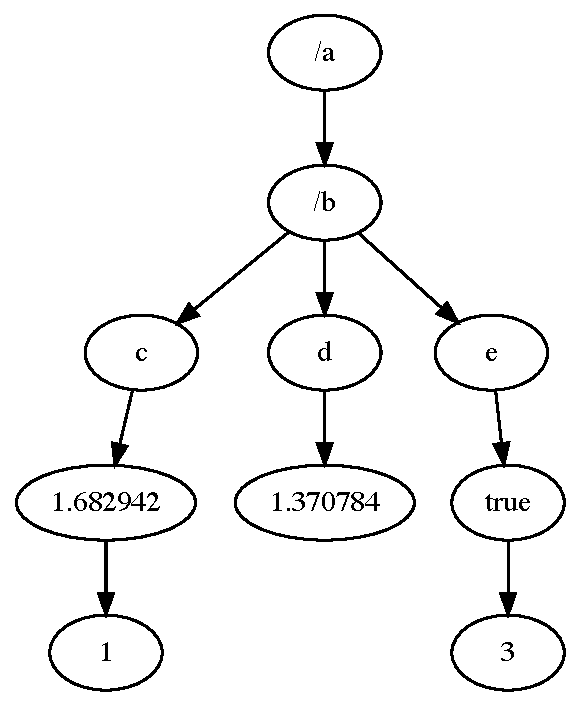
\includegraphics[width=0.5\columnwidth]{eval/sample3}
\caption{Tree generated by evaluation of the mathematical operations in Figure \ref{parsesample2}.}
\label{treesample2}
\end{center}
\end{figure}


%---------------------------
\subsubsection{Selectors}

A selector is a tree that takes the following form:
\code{? condition, if\_true, if\_false}
It selects one of the two branches according to the Boolean value of the \emph {condition}.

\exemple
\code{? true, 1, 0; \ \  $\Rightarrow$ $t := 1\ [\nulltree]$}


%---------------------------
\subsection{Variables}

A variable is the association of an identifier and a tree. Its general form is
$varname = t$

\exemple
\code{foo = /A/B (x 0), (y 1); }

%---------------------------
\subsubsection{Evaluation}

The evaluation of a variable consists in expanding the tree represented by this variable at its current position.
Let the tree $t$ and the variable $var$ be defined as follows:
\op{t :=  v f\\
var = t
}
The evaluation of $var$ in the context of a tree $t'$ is defined as:
\op{t'$_{\{var\}}$ :=  \$var f' $\Rightarrow$ t" := t \seq\ \toforet(t') \\
where \\
\toforet(t := v f) $\Rightarrow$ t' := \foret\ f
}
t'$_{\{var\}}$ denotes a tree whose environment contains the variable $var$.


\exemple
\code{x = x 0;\\
y = y 0;\\
/A/B \$x, \$y; \ \ $\Rightarrow$  /A/B (x 0), (y 1);}


%---------------------------
\subsubsection{Local Environnements}

Each tree is evaluated in an environment containing the list of all the variables of its parent. However, a variable can be evaluated in a local environment, which is defined as:
\code{var = t;\\
\$var\{a=t1, b=t2,\etc\} \ \ $\Rightarrow$  t' := t$_{\{a, b,\etc\}}$}



%---------------------------
\subsection{Nodes in Intention}

A \emph{node in intention} is a compact description of a forest. It can also be seen as a \emph{loop} control structure. The general form is as follows:
\begin{description}
 \setlength\itemsep{0.0em}
\item $id[n…m]$ 	where $n$ and $m$ are integers
\item $id[ab…xy]$ where $a,b,x,y$ are letters.
\end{description}

Expanding a node in intention transforms that node into a forest. We will note \nexpand\ the expansion operation:
\code{\nexpand(id[n…m]) \ $\Rightarrow$ \foret [id$n$,id$n+1$,…,id$m$]\\
\\
\nexpand(id[ab…xy]) $\Rightarrow$ \foret [id$ab$,id$ac$,…,id$ay$,\\
\ulc id$bb$,id$bc$,…,id$by$,\\
\ulc …,\\
\ulc id$xb$,id$xc$,…,id$xy$]
}

%---------------------------
\subsubsection{Special Forms}

A \emph{node in intention} can take the following special forms: 
\begin{description}
\item $id[i:n…m]$ 	where $i$ is an identifier
\item $id[i:j:ab…xy]$ where $i,j$ are identifiers.
\end{description}
These identifiers denote variables that are instantiated in the environment by the expansion operation, with the current index value:
\code{\nexpand(id[i:n…m]) \\
\ $\Rightarrow$ \foret [id$n_{\{i=0\}}$,id$n+1_{\{i=1\}}$,…,id$m_{\{i=m-n\}}$]\\
\\
\nexpand(id[i:j:ab…xy]) \\
\ $\Rightarrow$ \foret [id$ab_{\{i=0,j=0\}}$,…,id$ay_{\{i=y-b,j=0\}}$,\\
\uld id$bb_{\{i=0,j=1\}}$,…,id$by_{\{i=y-b,j=1\}}$,\\
\uld …,\\
\uld id$xb_{\{i=0,j=x-a\}}$…,id$xy_{\{i=y-b,j=x-a\}}$]
}

\exemple

Figure \ref{treesample3} shows a script making use of a node in intention with the corresponding evaluated tree.

\begin{figure}[htbp]
\code{/a/b[i:1...3] x (- (* \$i, 0.5), 0.5);}
\begin{center}
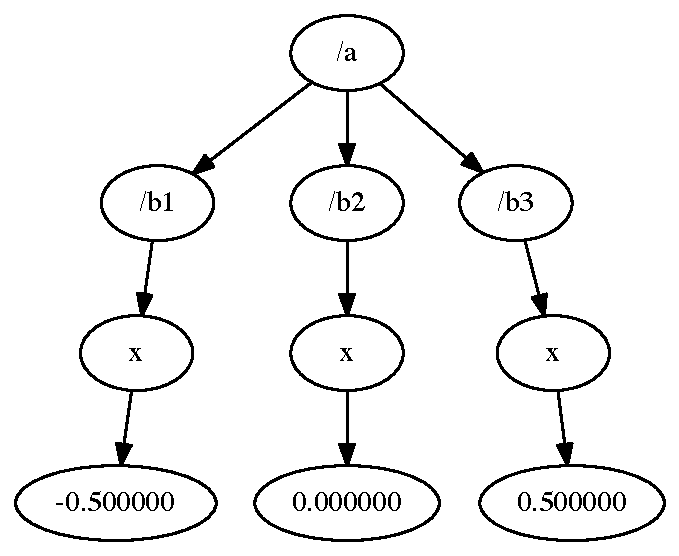
\includegraphics[width=0.6\columnwidth]{eval/sample2}
\caption{Tree generated by the expansion and the evaluation of the above script.}
\label{treesample3}
\end{center}
\end{figure}

%---------------------------
\subsection{Slash (/)}\label{ssec:slash}

The \emph{slash} nodes are used to transform a tree into OSC messages. Their purpose is to discriminate the OSC address and the parameters of the message. Transforming a tree into OSC messages consists in enumerating all the paths from the root node up to the first parameter, which is the first node that is not preceded by a \emph{slash}.



%-------------------------------------------------
\section{Example}

The script below presents an example of the new version of the \IS\ scripting language. Variables are indicated in blue. Local variables are declared in red.

\lstdefinelanguage{inscore} 
{
classoffset=0,
morekeywords={}, keywordstyle=\color{blue},
classoffset=1,
morekeywords={addr, count, radius, size, pos, color }, keywordstyle=\color{red},
classoffset=2,
keywordsprefix=$,
sensitive=true,
morecomment=[l]{\#},
morestring=[b]", 
}

\lstset{backgroundcolor=\color{lightgrey}, extendedchars=true, inputencoding=utf8}

\begin{lstlisting}[language=inscore, extendedchars=true, basicstyle=\small\ttfamily]
# variables declaration 
pi    = 3.141592653589793;

# the next variables make use of 'count'
# a variable that is instanciated locally
step  = / ( * 2, $pi), $count;
hstep = / 0.3, $count;

x = math.sin ( * $step, (+ $i, $pos));
y = math.cos ( * $step, (+ $i, $pos));

hue    = (+ $color, (* $hstep, $i));
bstart = 0.4;
bstep  = / (- 1, $bstart), $count;
brigthness= + $bstart, (* $bstep, $i);

# this is a classical OSC message
# that simply clears the scene
/ITL/scene/* del;

# this is the main variable. It will be
# expanded to create a series of objects.
# Most of the variables are locally defined.  
circle = (/ITL/scene/$addr  
          (set ellipse $size $size),
          (x * $x, $radius),
          (y * $y, $radius),
          (hsb $hue, $brigthness,1.));

# finally the 'circle' variable is used
# with different parameters. 
$circle{addr=c1_[i:1...30],count=30, 
   radius=0.7,size=0.1,pos=0,color=0.};
$circle{addr=c2_[i:1...24],count=24,
   radius=0.5,size=0.08,pos=6,color=0.1};
$circle{addr=c3_[i:1...20],count=20,
   radius=0.3,size=0.06,pos=10,color=0.2};
$circle{addr=c4_[i:1...12],count=12,
   radius=0.15,size=0.045,pos=9,color=0.35};

\end{lstlisting}


Evaluation of this script produces OSC messages fully compatible with the previous version of the language, and which are schematically presented below. 
\code[1]{/ITL/scene/c1\_1 set ellipse 0.1 0.1;\\
/ITL/scene/c1\_1 x 0.0;\\
/ITL/scene/c1\_1 y 0.7;\\
/ITL/scene/c1\_1 hsb 0.0 0.4 1.;\\
/ITL/scene/c1\_2 set ellipse 0.1 0.1;\\
/ITL/scene/c1\_2 x 0.145538;\\
/ITL/scene/c1\_2 y 0.684704;\\
/ITL/scene/c1\_2 hsb 0.01 0.42 1.;\\
...\\
...\\
/ITL/scene/c4\_12 set ellipse 0.045 0.045;\\
/ITL/scene/c4\_12 x -0.129904;\\
/ITL/scene/c4\_12 y -0.074999;\\
/ITL/scene/c4\_12 hsb 0.625 0.95 1.;
}

In practice, this example expresses the scene illustrated by the Figure \ref{samplescene} in 20 lines, where 345 lines were necessary in the previous version of the language.  

\begin{figure}[htbp]
\begin{center}
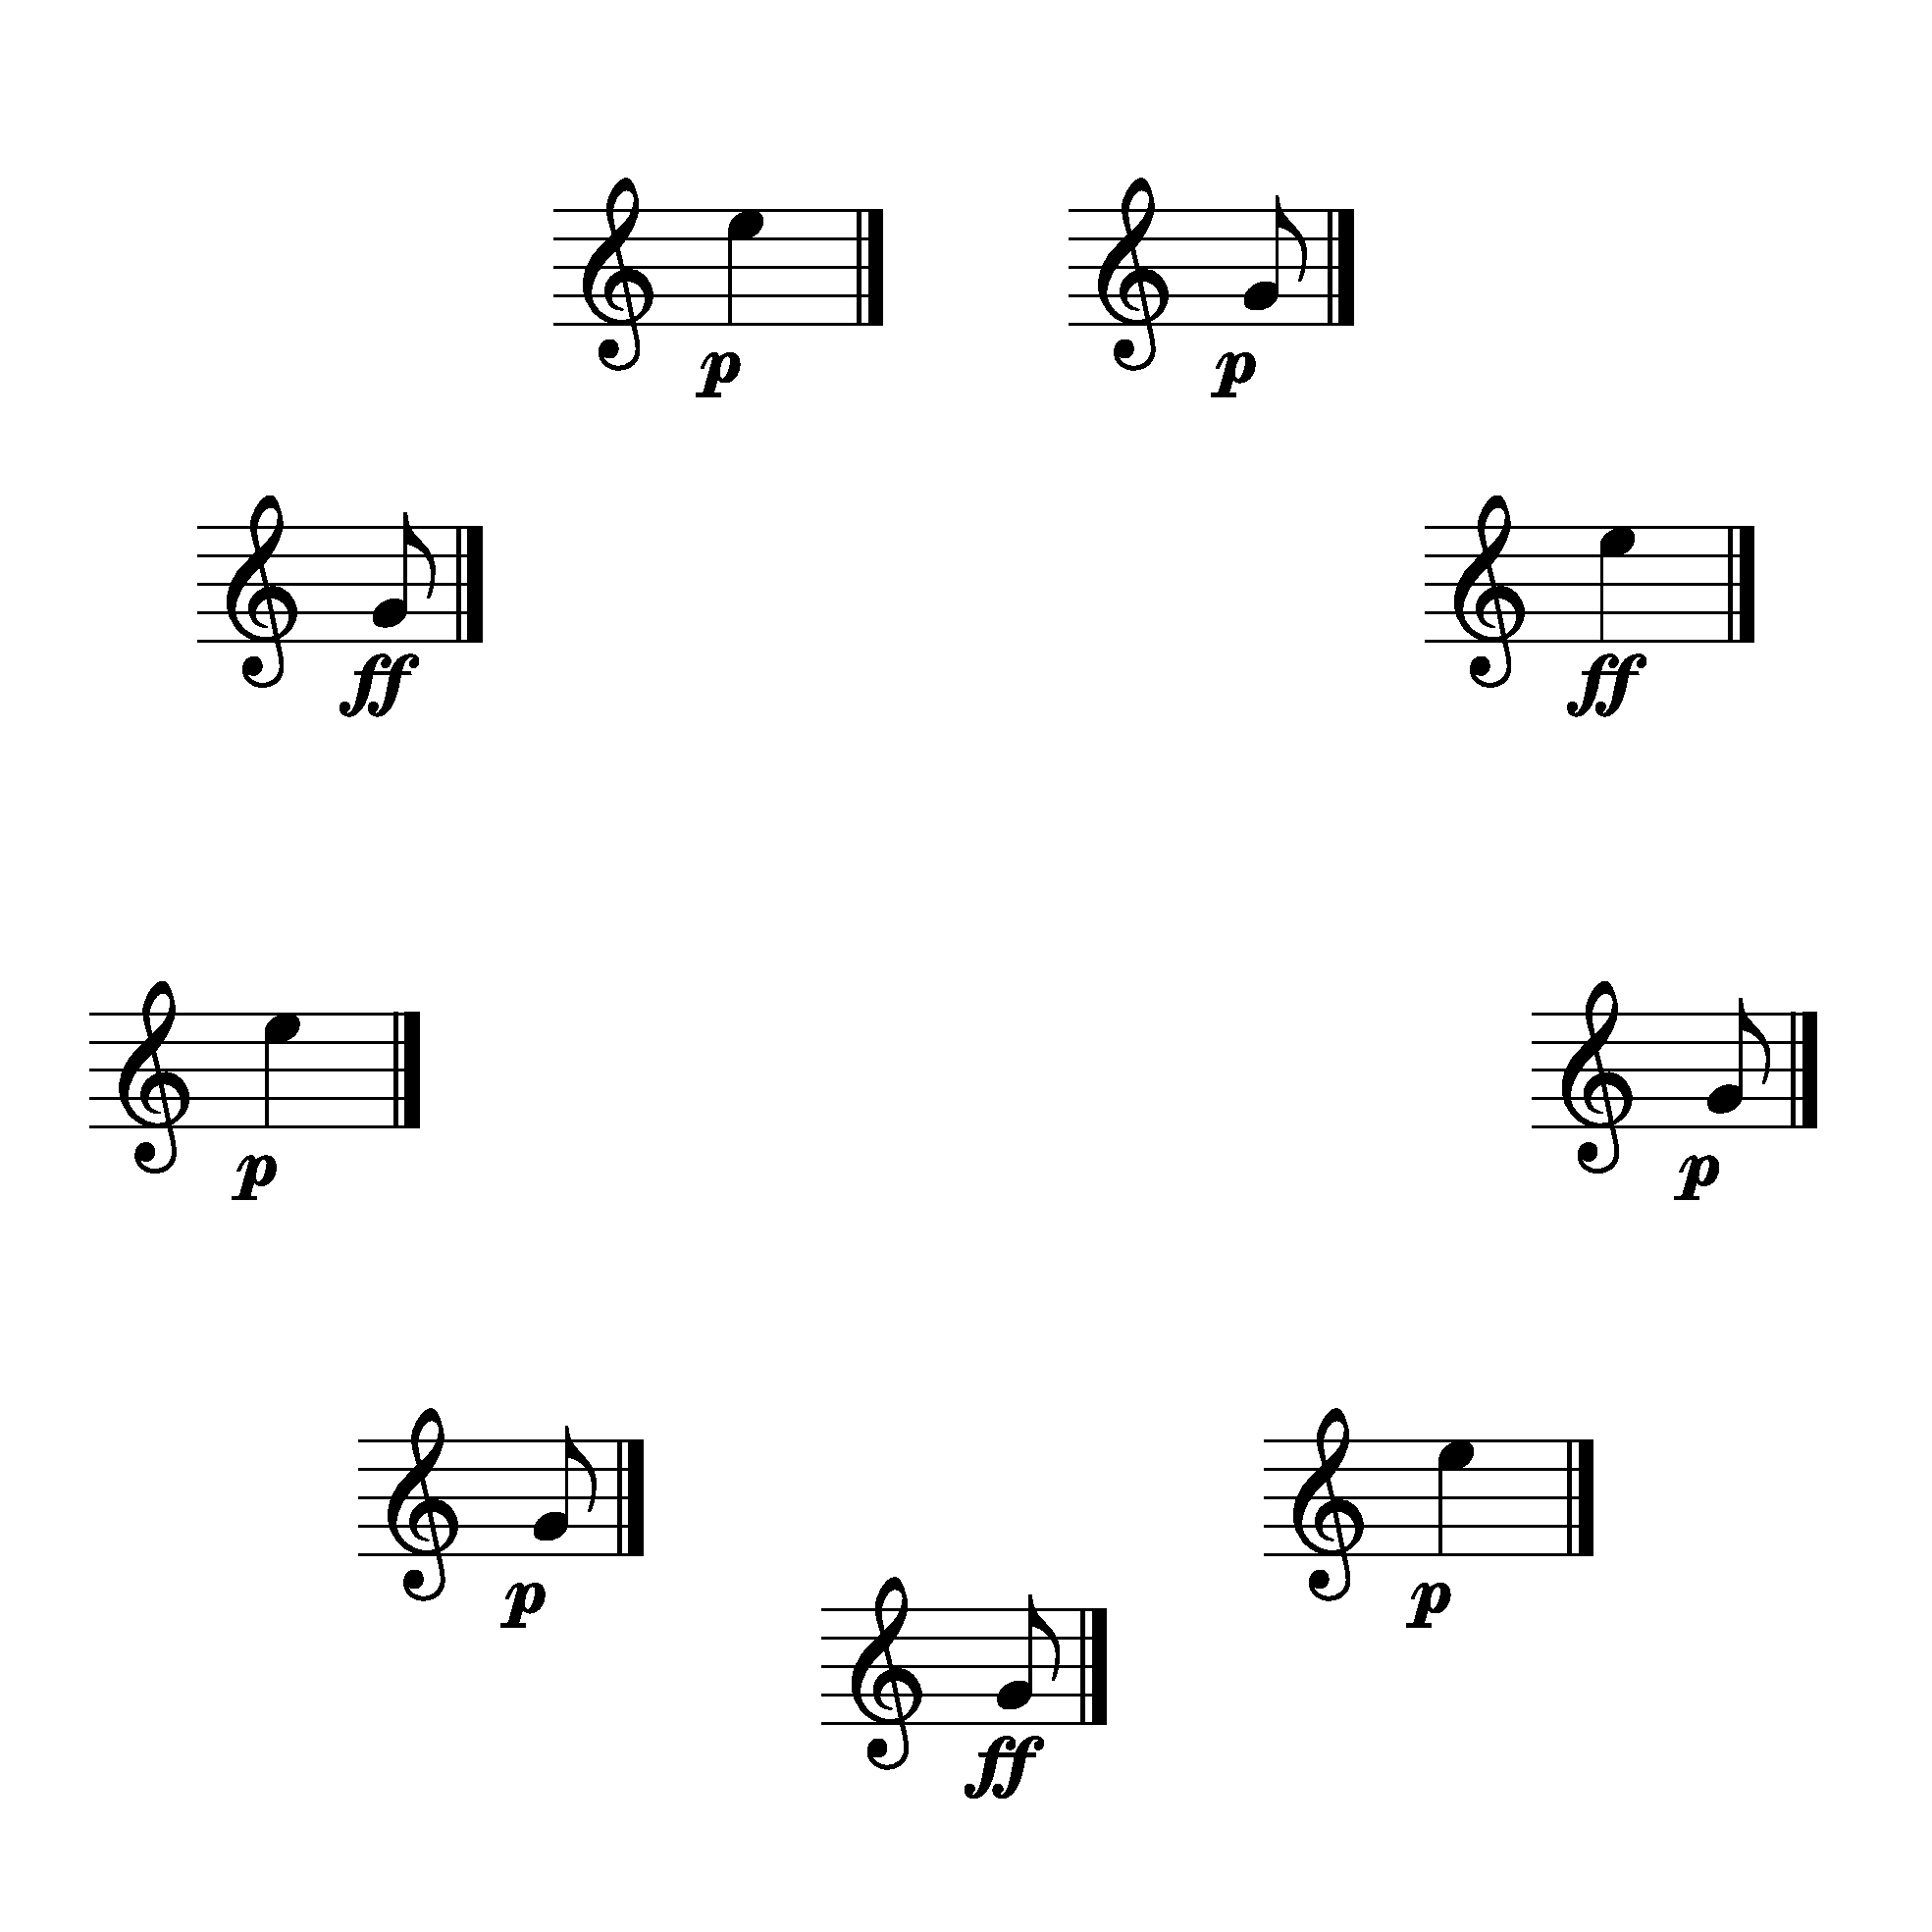
\includegraphics[width=0.8\columnwidth]{scene}
\caption{\IS\ scene corresponding to the sample script.}
\label{samplescene}
\end{center}
\end{figure}


%-------------------------------------------------
\section{Conclusions}
From two elementary operations on trees - sequencing and parallelisation - we have homogeneously introduced the notions of variables and of mathematical and logical operations on trees. The resulting language is much more expressive than the  previous version of the \IS\ scripting language. 
It supports parallelisation of the arguments of a message, variables to describe addresses, series of addresses expressed in a concise manner, use of local variables allowing reusing scripts or parts of scripts in different contexts.



%%%%%%%%%%%%%%%%%%%%%%%%%%%%%%%%%%%%%%%%%%%%%%%%%%%%%%%%%%%%%%%%%%%%%%%%%%%%%
%bibliography here
\balance
\bibliography{../interlude}

\end{document}
